\chapter{Supersymmetry and the MSSM}

In recent years it has already been seen that the standard model 
performs well in describing experimental observations at energies around
the electroweak scale of $O(246 \GeV)$.
The recent discovery of a standard model-like higgs boson brings with it
more confidence of the model. Questions arise when this model is seen as 
a part of a grand unified theory, for example, what happens when we probe
regions between the electroweak and planck scales $O(1.22 \times10^{19} \GeV)$? 
The standard model encounters difficulties in renormalization, this is known
as the Hierarchy Problem.

To illustrate these divergences we consider the radiative corrections to the higgs mass
from a fermion loop.
As seen in the previous chapter, the potential of the standard model higgs field can be
written as, 
\begin{equation}
V= \mu^{2}|\phi|^{2}+\lambda|\phi|^{4}
\end{equation}
where $\phi$ is a complex scalar field.
A non-vanishing vacuum expectation value of $246 \GeV$ is required to derive the masses of the $W/Z$
and the mass of the higgs which is defined as, $m_{h}=\sqrt{2\lambda v^{2}}$.

%When considering, for example, higher order radiative corrections to the mass of the higgs. For example, 
A fermion loop correction, seen in figure \ref{fig:fermionLoop}, 
adds the term $-\lambda_{f}\phi \bar{f}f$ to the Lagrangian.
This manifests as a correction to the higgs mass, namely,
\begin{equation}
\Delta m_{H}^{2}=-\frac{|\lambda_{f}|^{2}}{8\pi^{2}}\Lambda_{UV}^{2}+...
\label{eq:SUS1}
\end{equation}
%The loops represent terms which are proportional to $m_{f}^{2}$.
Where $\Lambda_{UV}$ is the ultraviolet cutoff. %%define UV cutoff
Then what happens when higher energy scales are considered and $\Lambda_{UV}\rightarrow \inf$?
Since the standard model is a renormalizable theory one could simply
pick $\Lambda_{UV}$ so that it regulates the loop. However, this would imply
that $\Lambda_{UV}$ is the energy scale at which new physics should enter.
To make matters worse, there are quantum corrections from the radiative
effects of every particle that couples to the higgs. If each of these 
particles gain their mass through the higgs mechanism then the entire standard model 
mass spectrum is sensitive to $\Lambda_{UV}$!

\section{Motivations for Supersymmetry}
To solve the Hierarchy Problem suppose there exists a massive scalar particle S, 
of mass $m_{S}$, that couples
to the higgs with a term $-\lambda_{S}\phi^{2} S^{2}$ as seen is 
figure \ref{fig:scalarLoop}. This massive scalar would give a correction of,
\begin{equation}
\Delta m_{H}^{2}=\frac{\lambda_{s}}{16\pi^{2}}\left[\Lambda_{UV}^{2}-2m_{s}^{2}ln(\Lambda_{UV}/m_{S})+... \right].
\label{eq:SUS2}
\end{equation}
By examining (\ref{eq:SUS1}) and (\ref{eq:SUS2}) it is apparent that if each of the quarks
and leptons is accompanied by a complex scalar with $\lambda_{S}=|\lambda_{f}|^{2}$  %OR TWO??
then the $\Lambda_{UV}^{2}$ terms will cancel. This model of symmetry between bosons
and fermions is known as supersymmetry (SUSY).

\begin{figure}[hb]
  \centering
  \begin{subfigure}[trim = 0mm 0mm 0mm 0mm, clip, width=3cm]{.4\textwidth}
	\marginbox{0mm 0pt 0mm 0pt}{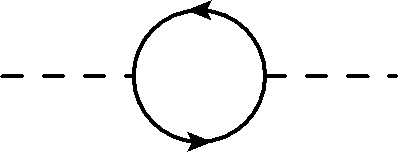
\includegraphics[width=\textwidth]{images/fermionLoop.png}}
                %\marginbox{-10mm 0pt 10mm 0pt}{}
                \caption{}
                \label{fig:fermionLoop}
\end{subfigure}
\begin{subfigure}[trim = 0mm 0mm 0mm 0mm, clip, width=3cm]{.4\textwidth}
	\marginbox{0mm 0pt 0mm 0pt}{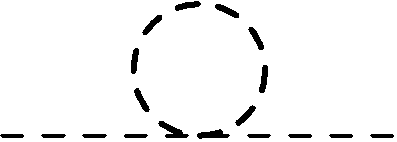
\includegraphics[width=\textwidth]{images/SLoop.png}}
	\caption{}
                %\marginbox{10mm 0pt -10mm 0pt}{}
                \label{fig:scalarLoop}
                	
  \end{subfigure}
   \caption[]{One loop quantum corrections for a fermion (\ref{fig:scalarLoop}) and a scalar (\ref{fig:scalarLoop}). }
\end{figure}

To define SUSY a set of generators which 
transforms a fermionic state into a bosonic state and vice versa is needed. The simplest 
operator which can perform these operations is a 2 component Weyl spinor $Q$
such that,
\begin{equation}
Q|\mathrm{Boson}\rangle=|\mathrm{Fermion}\rangle \qquad Q|\mathrm{Fermion}\rangle=|\mathrm{Boson}\rangle
\end{equation}.
The generators $Q$ and $Q^{\dagger}$ must obey the anticommutation
and commutation algebra,
\begin{equation}
\{Q,Q^{\dagger}\}=P^{\mu}
\end{equation}
\begin{equation}
\{Q,Q\}=\{Q^{\dagger},Q^{\dagger}\}=0
\end{equation}
\begin{equation}
[P^{\mu},Q ]=[P^{\mu},Q^{\dagger}]=0
\end{equation}.
where $P^{\mu}$ is the generator of space-time translations.

In the supersymmetric model the SM and SUSY particles are arranged
into supermultiplets. These supermultiplets must contain both the SM fermion
and the boson superpartner. In the simplest approach, a  spin $\frac{1}{2}$
weyl fermion (for example, $e$) must have %%%check this
a spin-0 superpartner $\tilde{e}$, likewise, a supermultiplet with a spin-1 gauge boson ($W$) would have
 a spin $\frac{1}{2}$ weyl fermion superpartner ($\tilde{W}$).
The naming convention for super particles calls for the names of
the fermionic standard model particles to be prepended by an 's', for example, 
'selectron' is short of 'scalar electron'; the gauge bosons are appended
with an 'ino', for example a 'wino'. If SUSY remained unbroken
then $m_{e}$ bust be equal to $m_{\tilde{e}}$. Since sparticles like $\tilde{e}$ have not 
yet been discovered this implies that SUSY must be a broken
symmetry.

\section{Higgs Sector of the MSSM}
The most simple supersymmetric extension of the standard model is the MSSM.
In the MSSM two higgs doublets with an $SU(2)_{L}$ symmetry,
\begin{equation}
\Phi_{1}=
\left(
    \begin{array}{c}
      \phi_{1}^{0*} \\
      -\phi_{1}^{-}
    \end{array}
  \right) 
 \qquad
\Phi_{2}=
\left(
    \begin{array}{c}
      \phi_{2}^{+} \\
      -\phi_{2}^{0}
    \end{array}
  \right), 
  \label{eq:SUSYhiggs}
\end{equation}
The $\Phi_{1}$ has a hypercharge of -1 and gives mass to each of the
down-type quarks and charged leptons whereas $\Phi_{2}$ gives masses
to the up-type quarks. The extra doublet
is needed to cancel out the corresponding supersymmetric higgs fermion
contributions.
$H_{1}^{0}$ and $H_{2}^{0}$ acquire vacuum expectation values $v_{1}$ and $v_{2}$ where
\begin{equation}
v = \sqrt{2}(v_{1}^{2}+v_{2}^{2})^{\frac{1}{2}}.
\end{equation}
The ratios of $v_{1}$ and $v_{2}$ is written as,
\begin{equation}
\tan(\beta)=\frac{v_{2}}{v_{1}}
\end{equation}
%%% something about shifting the neutral scalar fields by their vevs and diagonalization 
%The following higgs boson states are attained
Consequently the MSSM model has a total of five higgs bosons: two neutral higgs, h and H,
a pseudoscalar, A, and two charged higgs, $H^{\pm}$.
By translating the fields in (\ref{eq:SUSYhiggs}) to their minima and diagonalizing the matrix
the following higgs boson states are obtained,
\begin{equation}
\left(
    \begin{array}{c}
      H^{0}_{1} \\
     H^{0}_{2}
    \end{array}
  \right) 
  =
  \sqrt{2}
  \begin{pmatrix}
  \cos{\alpha} & \sin{\alpha}\\
  -\sin{\alpha}& \cos{\alpha}\\
  \end{pmatrix}
\left(
      \begin{array}{c}
      Re{\phi}_{1}^{0*}-v_{1} \\
     Re{\phi}_{2}^{0}-v_{2}
    \end{array}
  \right) 
\end{equation}
\begin{equation}
H_{3}^{0}=\sqrt{2}(\sin{\beta}Im\phi_{1}^{0*}+\cos{\beta}Im\phi^{0}_{2})
\end{equation}
\begin{equation}
H^{-}=(H^{+})^{*}=-\phi_{1}^{-}\sin{\beta}+\phi_{2}^{-}\cos{\beta}
\end{equation}

In the MSSM at tree level the number of independent parameters can be reduced to 3: $m_{W}$,
$\tan{\beta}$ and the mass of the pseudoscalar, $m_{A}$. The neutral boson masses are,
\begin{equation}
m_{h}^{2}=\frac{1}{2}\left(m_{A}^{2}+M_{Z}^{2}-\left[(m_{A}^{2}+
M_{Z}^{2})^{2}-4M_{Z}^{2}m_{A}^{2}\cos^{2}{(2\beta)}\right]^{\frac{1}{2}}\right)
\end{equation}
\nobreak
\begin{equation}
m_{H}^{2}=\frac{1}{2}\left(m_{A}^{2}+M_{Z}^{2}+\left[(m_{A}^{2}+
M_{Z}^{2})^{2}-4M_{Z}^{2}m_{A}^{2}\cos^{2}{(2\beta)}\right]^{\frac{1}{2}}\right).
\end{equation}
While the masses of the two charged bosons are,
\begin{equation}
m_{H^{\pm}}^{2}=m_{A}^{2}+M_{W}^{2}.
\end{equation}
In order to make reliable phenomenological predictions loop corrections must be included
which depend on the masses particles and free parameters of the SUSY model .
Due to the large number of free parameters,
searches for MSSM Higgs bosons are expressed in terms of benchmark scenarios where 
the lowest-order parameters tan$\beta$ and $M_A$ are varied, while fixing the other parameters that 
enter through radiative corrections to benchmark values. 
The $m_{h}^{\rm max}$ scenario~\cite{MHMAX-Carena,MHMAX-Carena-2002}
yields conservative expected limits in the tan$\beta$ and $M_A$ plane. 
%\linebreak[4]
\begin{center}
$
M_{SUSY} = 1 \mathrm{TeV}, 
\mu=-200 \mathrm{GeV}, 
$
\linebreak[4]
$
m_{\tilde{g}}=0.8 M_{SUSY}, 
M_{A} \leq 1000 \mathrm{GeV}, 
$
\linebreak[4]
$
X_{t}=2M_{SUSY}, 
A_{b} = A_{t}
$
%\linebreak[4]
\end{center}
Where 
$M_{SUSY}$ is the third generation squark mass parameter,
$\mu$ is the higgsino mass parameter,
$m_{\tilde{g}}$ is the gluino mass,
$X_{t}= A_{t}-\mu/\mathrm{tan}\beta$
$A_{b}$ denotes he Higgs-sbottom coupling and
$A_{t}$ is the trilinear Higgs-stop coupling.
The gaugino mass parameter, $M_{1}$, is fixed via the GUT relation,
\begin{equation} 
M_{1}=\frac{5\sin^{2}{\theta_{w}}}{3\cos^{2}{\theta_{w}}}M_{2}
\end{equation}
where $M_{2}$ is the SU(2)-gaugino mass parameter.
Results in this thesis are interpreted both in the context of the MSSM 
$m_{h}^{\rm max}$ scenario and also in a model independent way, 
in terms of upper limits on $\sigma\cdot$BR($A\slash H\slash h\rightarrow\Pgt\Pgt$) for 
gluon-fusion and b-associated neutral Higgs boson production.

\section{MSSM Higgs Production}

\begin{figure}[t]
\centering
  \begin{subfigure}[b]{.4\textwidth}
	\marginbox{-5mm 10pt 5mm 0pt}{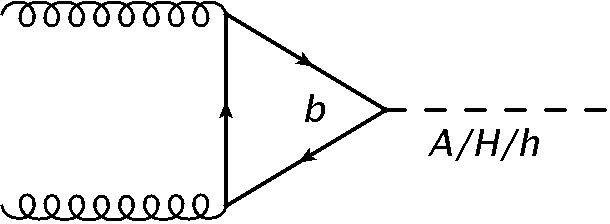
\includegraphics[width=\textwidth]{images/ggA.png} }
\caption[]{}
	\label{fig:ggA}
	\end{subfigure}	
   \begin{subfigure}[b]{.4\textwidth}
	\marginbox{5mm 0pt -5mm 0pt}{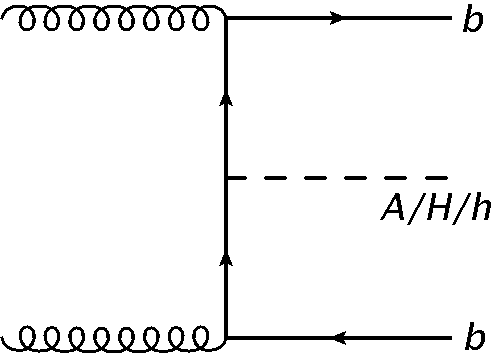
\includegraphics[width=\textwidth]{images/bbA.png}}

	\label{fig:bbA}

	\caption[]{}
    \end{subfigure}	
  	\caption[]
   	{MSSM Higgs Production diagrams}
	\label{fig:MSSMdiagrams}
\end{figure}
The two higgs doublet model of the MSSM is responsible for interesting
phenomenological effects which do not occur in the SM.
The dominant production mechanisms for the higgs particles are gluon
fusion and associated production of b quarks. 
The neutral MSSM Higgs boson production cross section
for small and moderate values of tan$\beta$ is high for 
gluon fusion ($gg\rightarrow A/H/h$) shown in figure (\ref{fig:ggA}). 

At large values of tan$\beta$ 
the b-associated production is the dominant contribution due to the enhanced bottom Yukawa 
coupling, therefore, associated production of b quarks with $A/H/h$ becomes a dominant signature.
Production of $gg\rightarrow A/H/h+bb$ is shown in figure (\ref{fig:MSSMdiagrams}b). 
Identification a b jet in the final state also serve to reduce futher unwanted backgrounds
such as $Z\rightarrow \Pgt\Pgt$. 
Figure (\ref{fig:tanbeta5}) shows cross sections for various MSSM higgs bosons 
and production mechanisms at a value of $\tan\beta=5$ and figure (\ref{fig:tanbeta5})
shows higgs bosons and production mechanisms at a value of $\tan\beta=30$.
Clearly, performing an analysis with and without b jet associated
production is useful for probing a larger region of MSSM phase space. Futhermore, due to the
enhanced couplings and the unique decay signatures the search for $A/H/h\rightarrow \Pgt\Pgt$
is at the LHC is of particular interest.

\begin{figure}[hb]
\centering
  \begin{subfigure}[b]{.4\textwidth}
	\marginbox{-5mm 10pt 5mm 0pt}{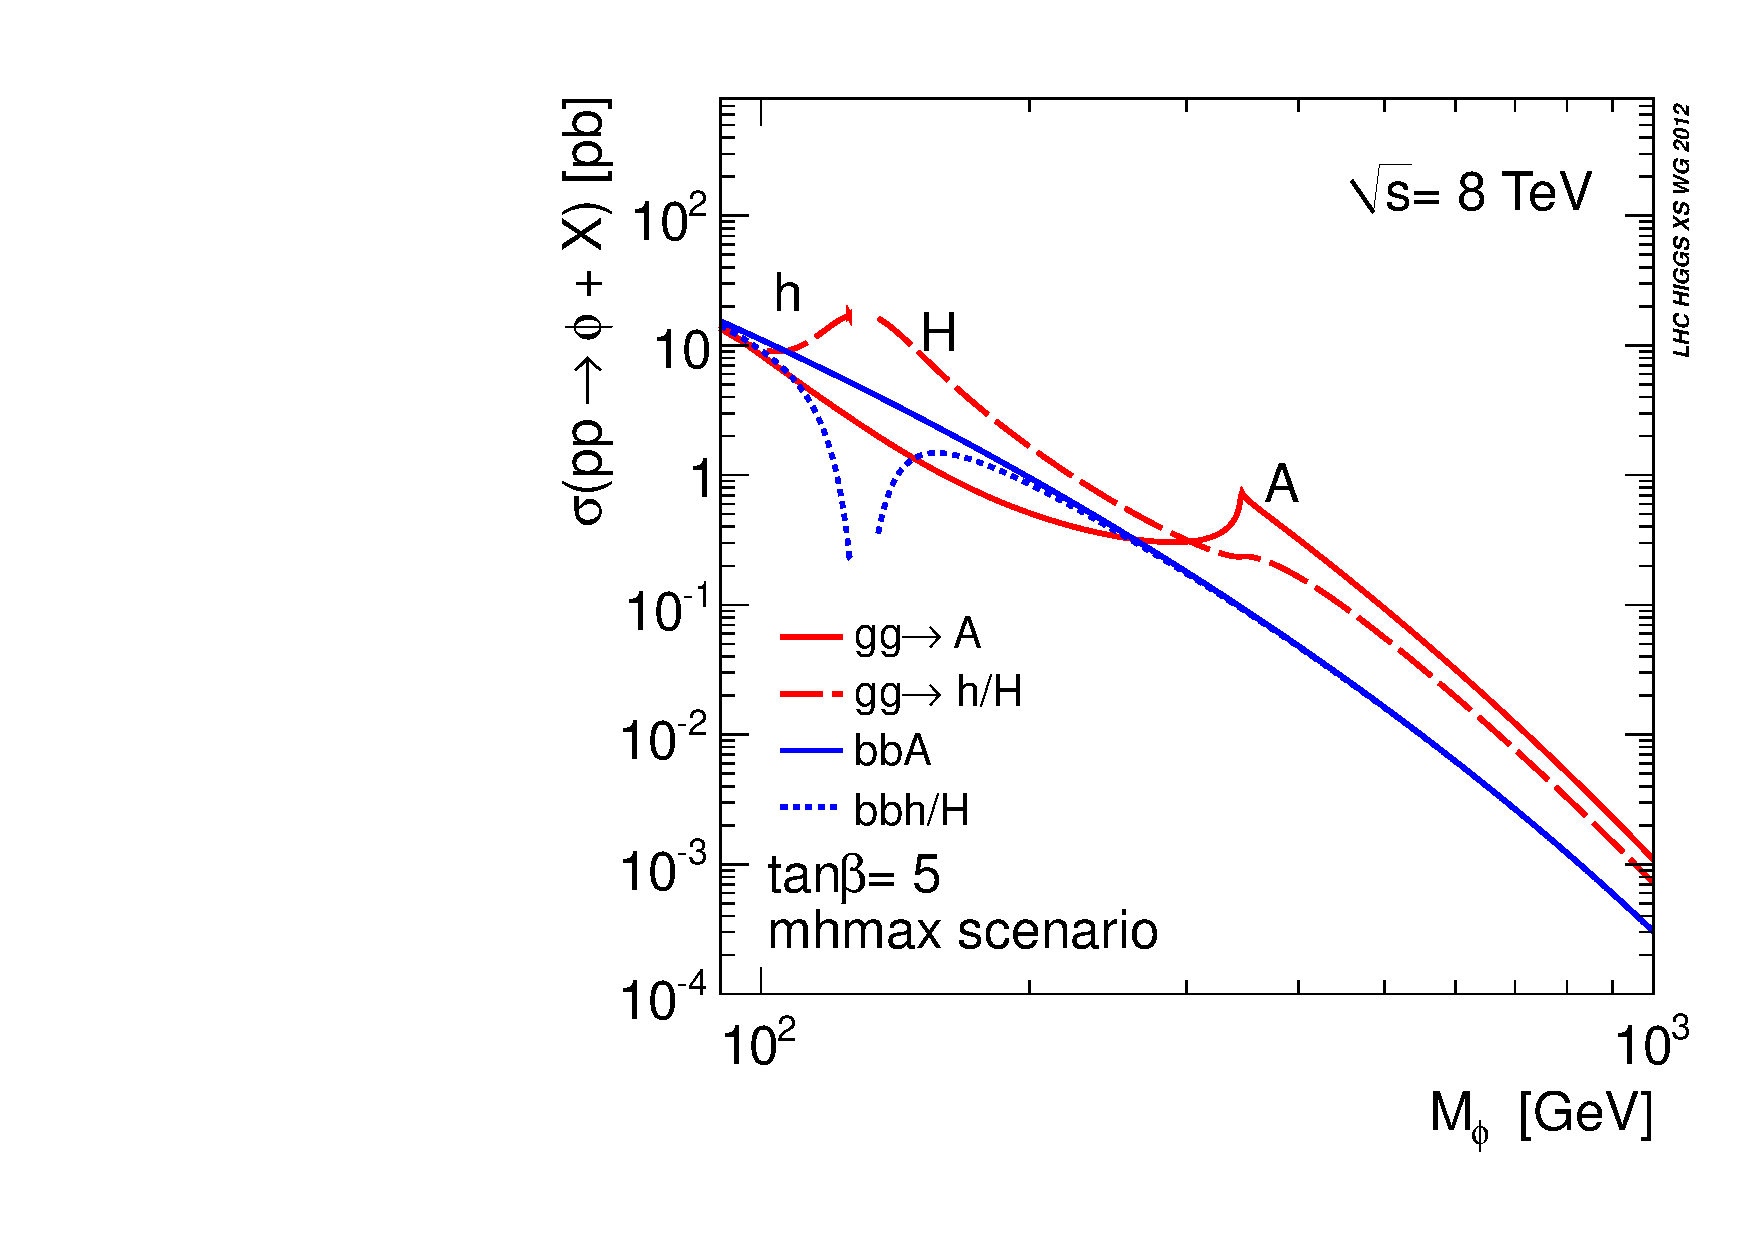
\includegraphics[width=\textwidth]{images/tanbeta5.pdf}}
	\label{fig:tanbeta5}
	\end{subfigure}	
   \begin{subfigure}[b]{.4\textwidth}
	\marginbox{5mm 0pt -5mm 0pt}{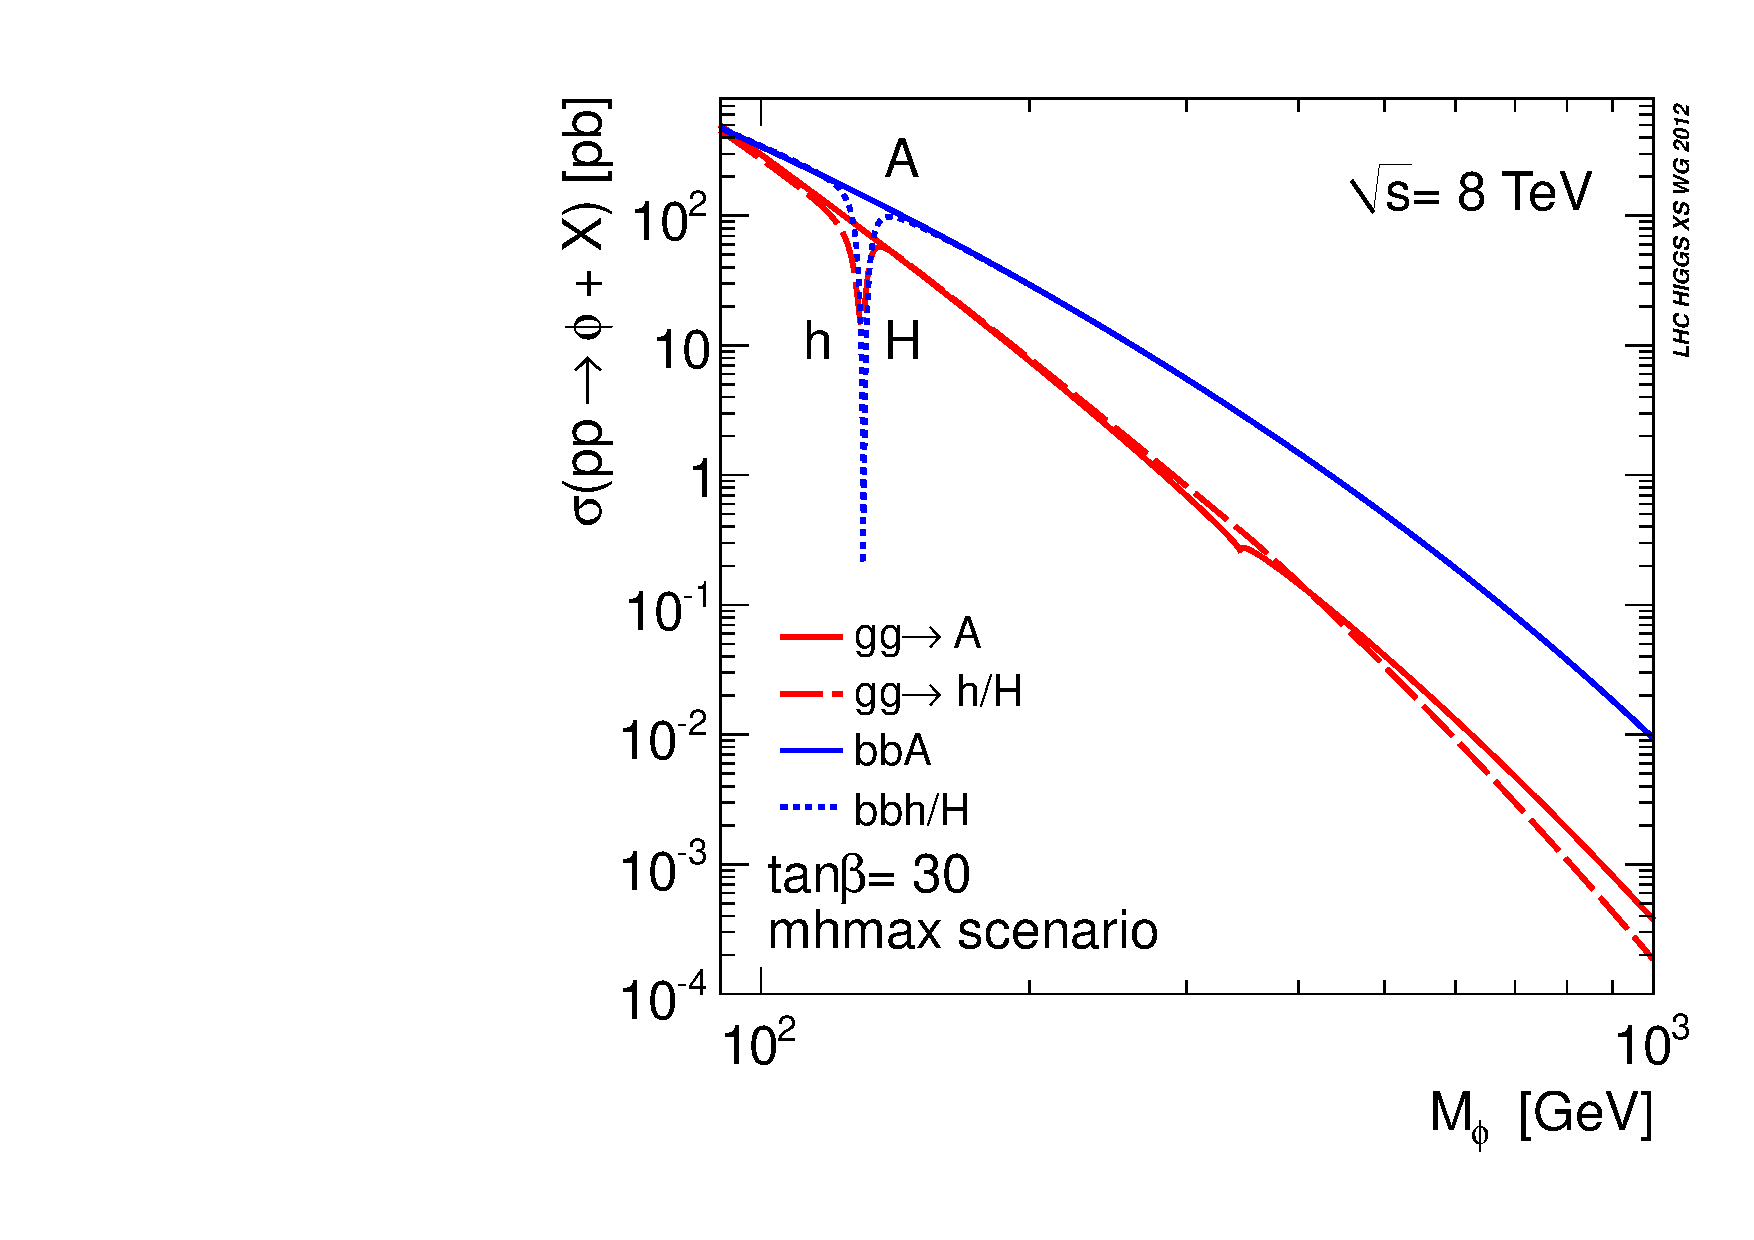
\includegraphics[width=\textwidth]{images/tanbeta30.pdf}}
	\label{fig:tanbeta30}
    \end{subfigure}	
  	\caption[]
   	{The cross sections for various MSSM higgs bosons and production 
	mechanisms at 8 TeV \cite{LHCHiggsCrossSectionWorkingGroup:2011ti}}
\end{figure}

%making the search for neutral MSSM Higgs bosons in the di-$\Pgt$ final state of particular interest. 
%In the region of large tan$\beta$, $O(10)$, the coupling to the heaviest down type fermions 
%$(b,\Pgt)$ is enhanced, 




